\documentclass[tikz]{standalone}

\pagestyle{empty}


\usepackage{amsmath}
\usepackage{tikz}
\usepackage{graphicx}
\usetikzlibrary{positioning,calc,fit,decorations.pathreplacing,arrows,positioning,backgrounds}

% Font settings:
\renewcommand{\familydefault}{\sfdefault}
\usepackage{pxfonts}
\newcommand{\figf}{\sffamily\bfseries\small} %Defines the font used for the labelling of figure panels.


% Color settings:
%\definecolor{hivc}{cmyk}{0,0.80,0.83,0.13}                %\definecolor{hivc}{HTML}{DE2D26}
\definecolor{hivc}{RGB}{24,116,205}
\definecolor{selfc}{cmyk}{0,0,0,0.6}                      %\colorlet{selfc}{gray!80!white}
\definecolor{Rblue}{RGB}{100,149,237}


\begin{document}
\scriptsize

% --------  FIGURE SATURATION
\begin{tikzpicture}[anchor=north west]
\clip (0,0) rectangle +(18,-10.5);



\begin{scope}[yshift=0cm]

	\node[anchor = north west] at (9,-0.3) {
		\includegraphics{../plots/F4panelB.pdf}
	};
	\node[anchor = north west] at (0,-0.3) {
		\includegraphics{../plots/F4panelA.pdf}
	};
	\node[anchor = north west] at (0,0) {\figf A};		
	\node[anchor = north west] at (9,0) {\figf B};	
\end{scope}


\begin{scope}[yshift=-8cm]

	\begin{scope}[xshift=2.1cm, yshift=-0.5cm]
		\filldraw[white] (0.05,0) rectangle +(2,-1);
		\begin{scope}[xshift=0,yshift=0.35cm]
			\clip (0.05,-0.25) rectangle +(1.5,-1.5);
			\node[anchor=north west,scale=0.5] at (0,0){
				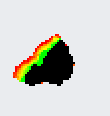
\includegraphics{../example-img/2D-m30l500b.png}
			};
		\end{scope}
		\begin{scope}[xshift=1.5cm,yshift=0.25cm]
			\clip (0.05,-0.15) rectangle +(1.5,-1.5);
			\node[anchor=north west,scale=0.5] at (0,0){
				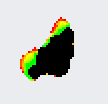
\includegraphics{../example-img/2D-m30l500.png}
			};
		\end{scope}
		\draw (0.05,0.1) rectangle +(3,-1.5);
		\node[anchor = north] at (1.5,-1.4){protrusion splitting};
	\end{scope}
	
	\begin{scope}[xshift=5.6cm, yshift=-0.5cm]
		\filldraw[white] (0.05,0) rectangle +(2,-1);
		\begin{scope}[xshift=0,yshift=0.35cm]
			\clip (0.05,-0.25) rectangle +(1.5,-1.5);
			\node[anchor=north west,scale=0.5] at (-0.2,0){
				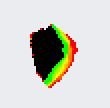
\includegraphics{../example-img/2D-m100-l60.png}
			};
		\end{scope}
		\begin{scope}[xshift=1.7cm,yshift=0.25cm]
			\clip (0.05,-0.15) rectangle +(1.5,-1.5);
			\node[anchor=north west,scale=0.5] at (-0.2,0){
				
\includegraphics{../example-img/2D-m100-l200.png}
			};
		\end{scope}
		\draw (0.05,0.1) rectangle +(1.5,-1.5);
		\draw (1.75,0.1) rectangle +(1.5,-1.5);
		\node[anchor = north] at (1.6,-1.4){angular diffusion};
	\end{scope}
	
	
	
	\begin{scope}[xshift=10.7cm, yshift=-0.5cm]
		\filldraw[white] (0.05,0) rectangle +(2,-1);
		\begin{scope}[xshift=0,yshift=0.35cm]
			%\clip (0.05,-0.25) rectangle +(1.5,-1.5);
			\node[anchor=north west,scale=0.13] at (-0.2,0){
				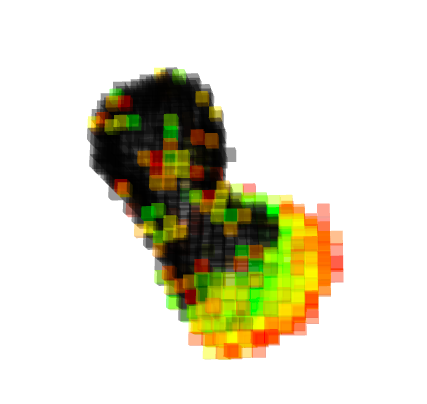
\includegraphics{../example-img/new3D-m30-l50.png}
			};
		\end{scope}
		\begin{scope}[xshift=1.7cm,yshift=0.25cm]
			%\clip (0.05,-0.15) rectangle +(1.5,-1.5);
			\node[anchor=north west,scale=0.13] at (-0.3,0){
				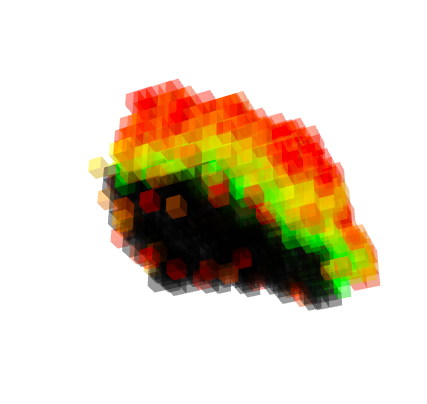
\includegraphics{../example-img/new3D-m30-l60.png}
			};
		\end{scope}
		\draw (0.05,0.1) rectangle +(1.5,-1.5);
		\draw (1.75,0.1) rectangle +(1.5,-1.5);
		\node[anchor = north] at (0.75,-1.4){unstable};
		\node[anchor = north] at (2.5,-1.4){stable};
	\end{scope}
	

	\begin{scope}[xshift=14.2cm, yshift=-0.5cm]
		\filldraw[white] (0.05,0) rectangle +(2,-1);
		\begin{scope}[xshift=0,yshift=0.35cm]
			\clip (0.05,-0.25) rectangle +(1.5,-1.5);
			\node[anchor=north west,scale=0.12] at (-0.2,-0.1){
				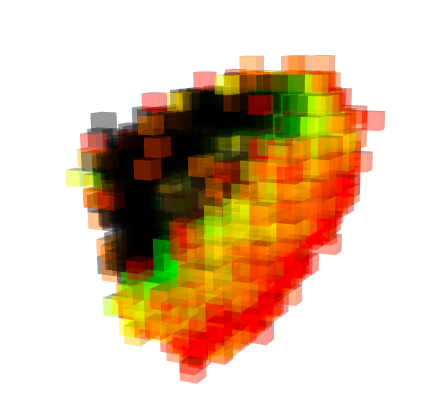
\includegraphics{../example-img/new3D-m50-l36b.png}
			};
		\end{scope}
		\begin{scope}[xshift=1.7cm,yshift=0.25cm]
			\clip (0.05,-0.15) rectangle +(1.5,-1.5);
			\node[anchor=north west,scale=0.12] at (-0.1,-0.1){
				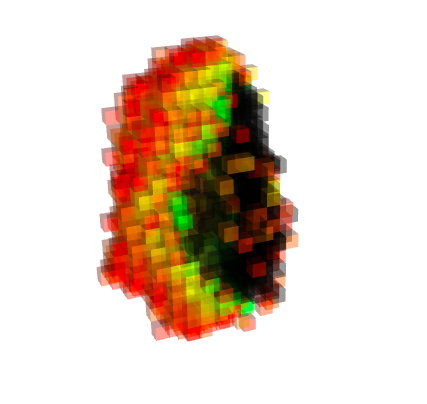
\includegraphics{../example-img/new3D-m50-l40.png}
			};
		\end{scope}
		\draw (0.05,0.1) rectangle +(1.5,-1.5);
		\draw (1.75,0.1) rectangle +(1.5,-1.5);
		\node[anchor = north] at (1.6,-1.4){angular diffusion};
	\end{scope}




	%\node[ anchor = north west ] at (0,0) {\figf C};
\end{scope}



\draw[dashed] (3.3,-1.3) -- +(0,-1.8);
\draw[dashed] (3.3,-3.7) -- +(0,-1.1);
\draw[dashed] (3.3,-5.3) -- +(0,-1.8);
\draw[dashed] (3.3,-7.7) -- +(0,-0.7);

\draw[dashed] (5.94,-1.3) -- +(0,-7.1);

\draw[dashed] (8.45,-1.3) -- +(0,-1.8);
\draw[dashed] (8.45,-3.7) -- +(0,-3.4);
%\draw[dashed] (8.75,-5.3) -- +(0,-1.8);
\draw[dashed] (8.45,-7.7) -- +(0,-0.7);


\draw[dashed] (12.38,-1.3) -- +(0,-1.8);
\draw[dashed] (12.38,-3.7) -- +(0,-1.1);
\draw[dashed] (12.38,-5.3) -- +(0,-1.8);
\draw[dashed] (12.38,-7.2) -- +(-0.9,-1.2);

\draw[dashed] (13.9,-1.3) -- +(0,-1.8);
\draw[dashed] (13.9,-3.7) -- +(0,-3.4);
\draw[dashed] (13.9,-7.7) -- +(0,-0.7);


\draw[dashed] (16.65,-1.3) -- +(0,-5.1);
\draw[dashed] (16.65,-6.4) -- +(-0.9,-2);

\draw[dashed] (17.44,-1.3) -- +(0,-1.8);
\draw[dashed] (17.44,-3.7) -- +(0,-3.4);
\draw[dashed] (17.44,-7.7) -- +(0,-0.7);

\end{tikzpicture}





\end{document}